\documentclass[border=10pt]{standalone}
\usepackage{tikz}
\usetikzlibrary{arrows.meta, shapes, positioning}

\begin{document}
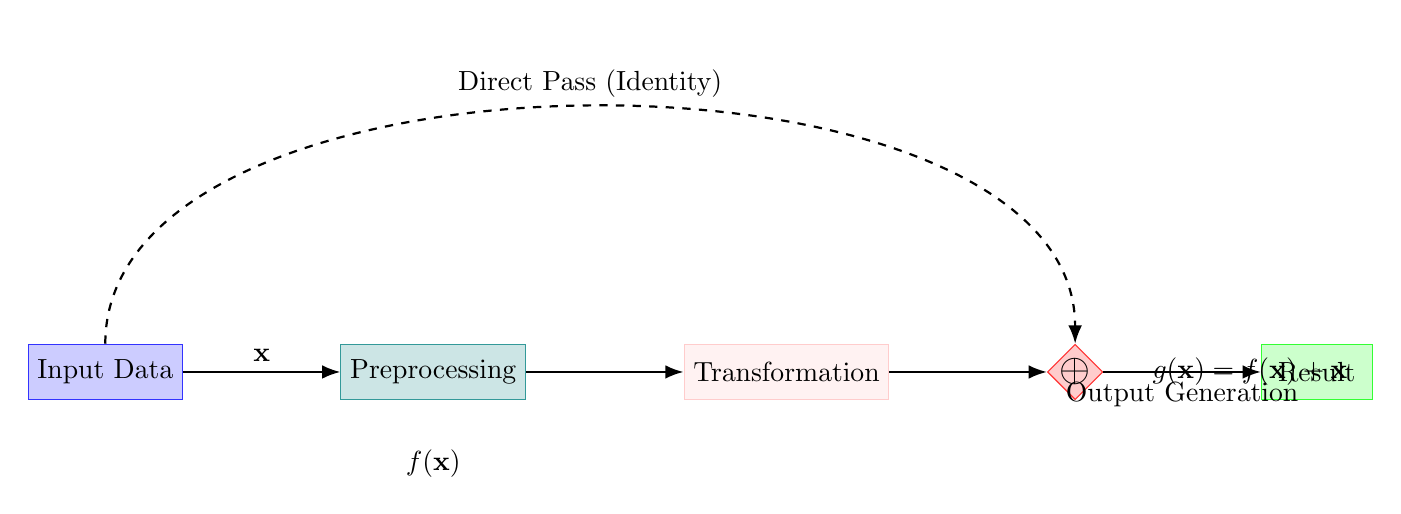
\begin{tikzpicture}[node distance=2cm, auto,
    block/.style={rectangle, draw=#1!80, fill=#1!20, minimum height=2em, minimum width=4em},
    sum/.style={diamond, draw=red!80, fill=red!20, minimum size=2em},
    arrow/.style={->, >=Latex, thick},
    dashedarrow/.style={->, >=Latex, dashed, thick}
]

% Nodes
\node[block=blue] (input) {Input Data};
\node[block=teal, right=of input] (preprocess) {Preprocessing};
\node[block=pink, right=of preprocess] (transform) {Transformation};
\node[sum, right=of transform] (add) {};
\node[block=green, right=of add] (result) {Result};

% Labels
\node[below=0.5cm of preprocess] (fx) {$f(\mathbf{x})$};
\node[right=0.5cm of add] (gx) {$g(\mathbf{x}) = f(\mathbf{x}) + \mathbf{x}$};

% Arrows
\draw[arrow] (input) -- node[above] {$\mathbf{x}$} (preprocess);
\draw[arrow] (preprocess) -- (transform);
\draw[arrow] (transform) -- (add);
\draw[arrow] (add) -- node[below] {Output Generation} (result);

% Direct Pass
\draw[dashedarrow] (input) to[out=90,in=90,distance=4cm] node[above] {Direct Pass (Identity)} (add);

% Addition Symbol
\node at (add.center) {\Large$\oplus$};

\end{tikzpicture}
\end{document}